\chapter{System tests}
\begin{figure}
        \centering
         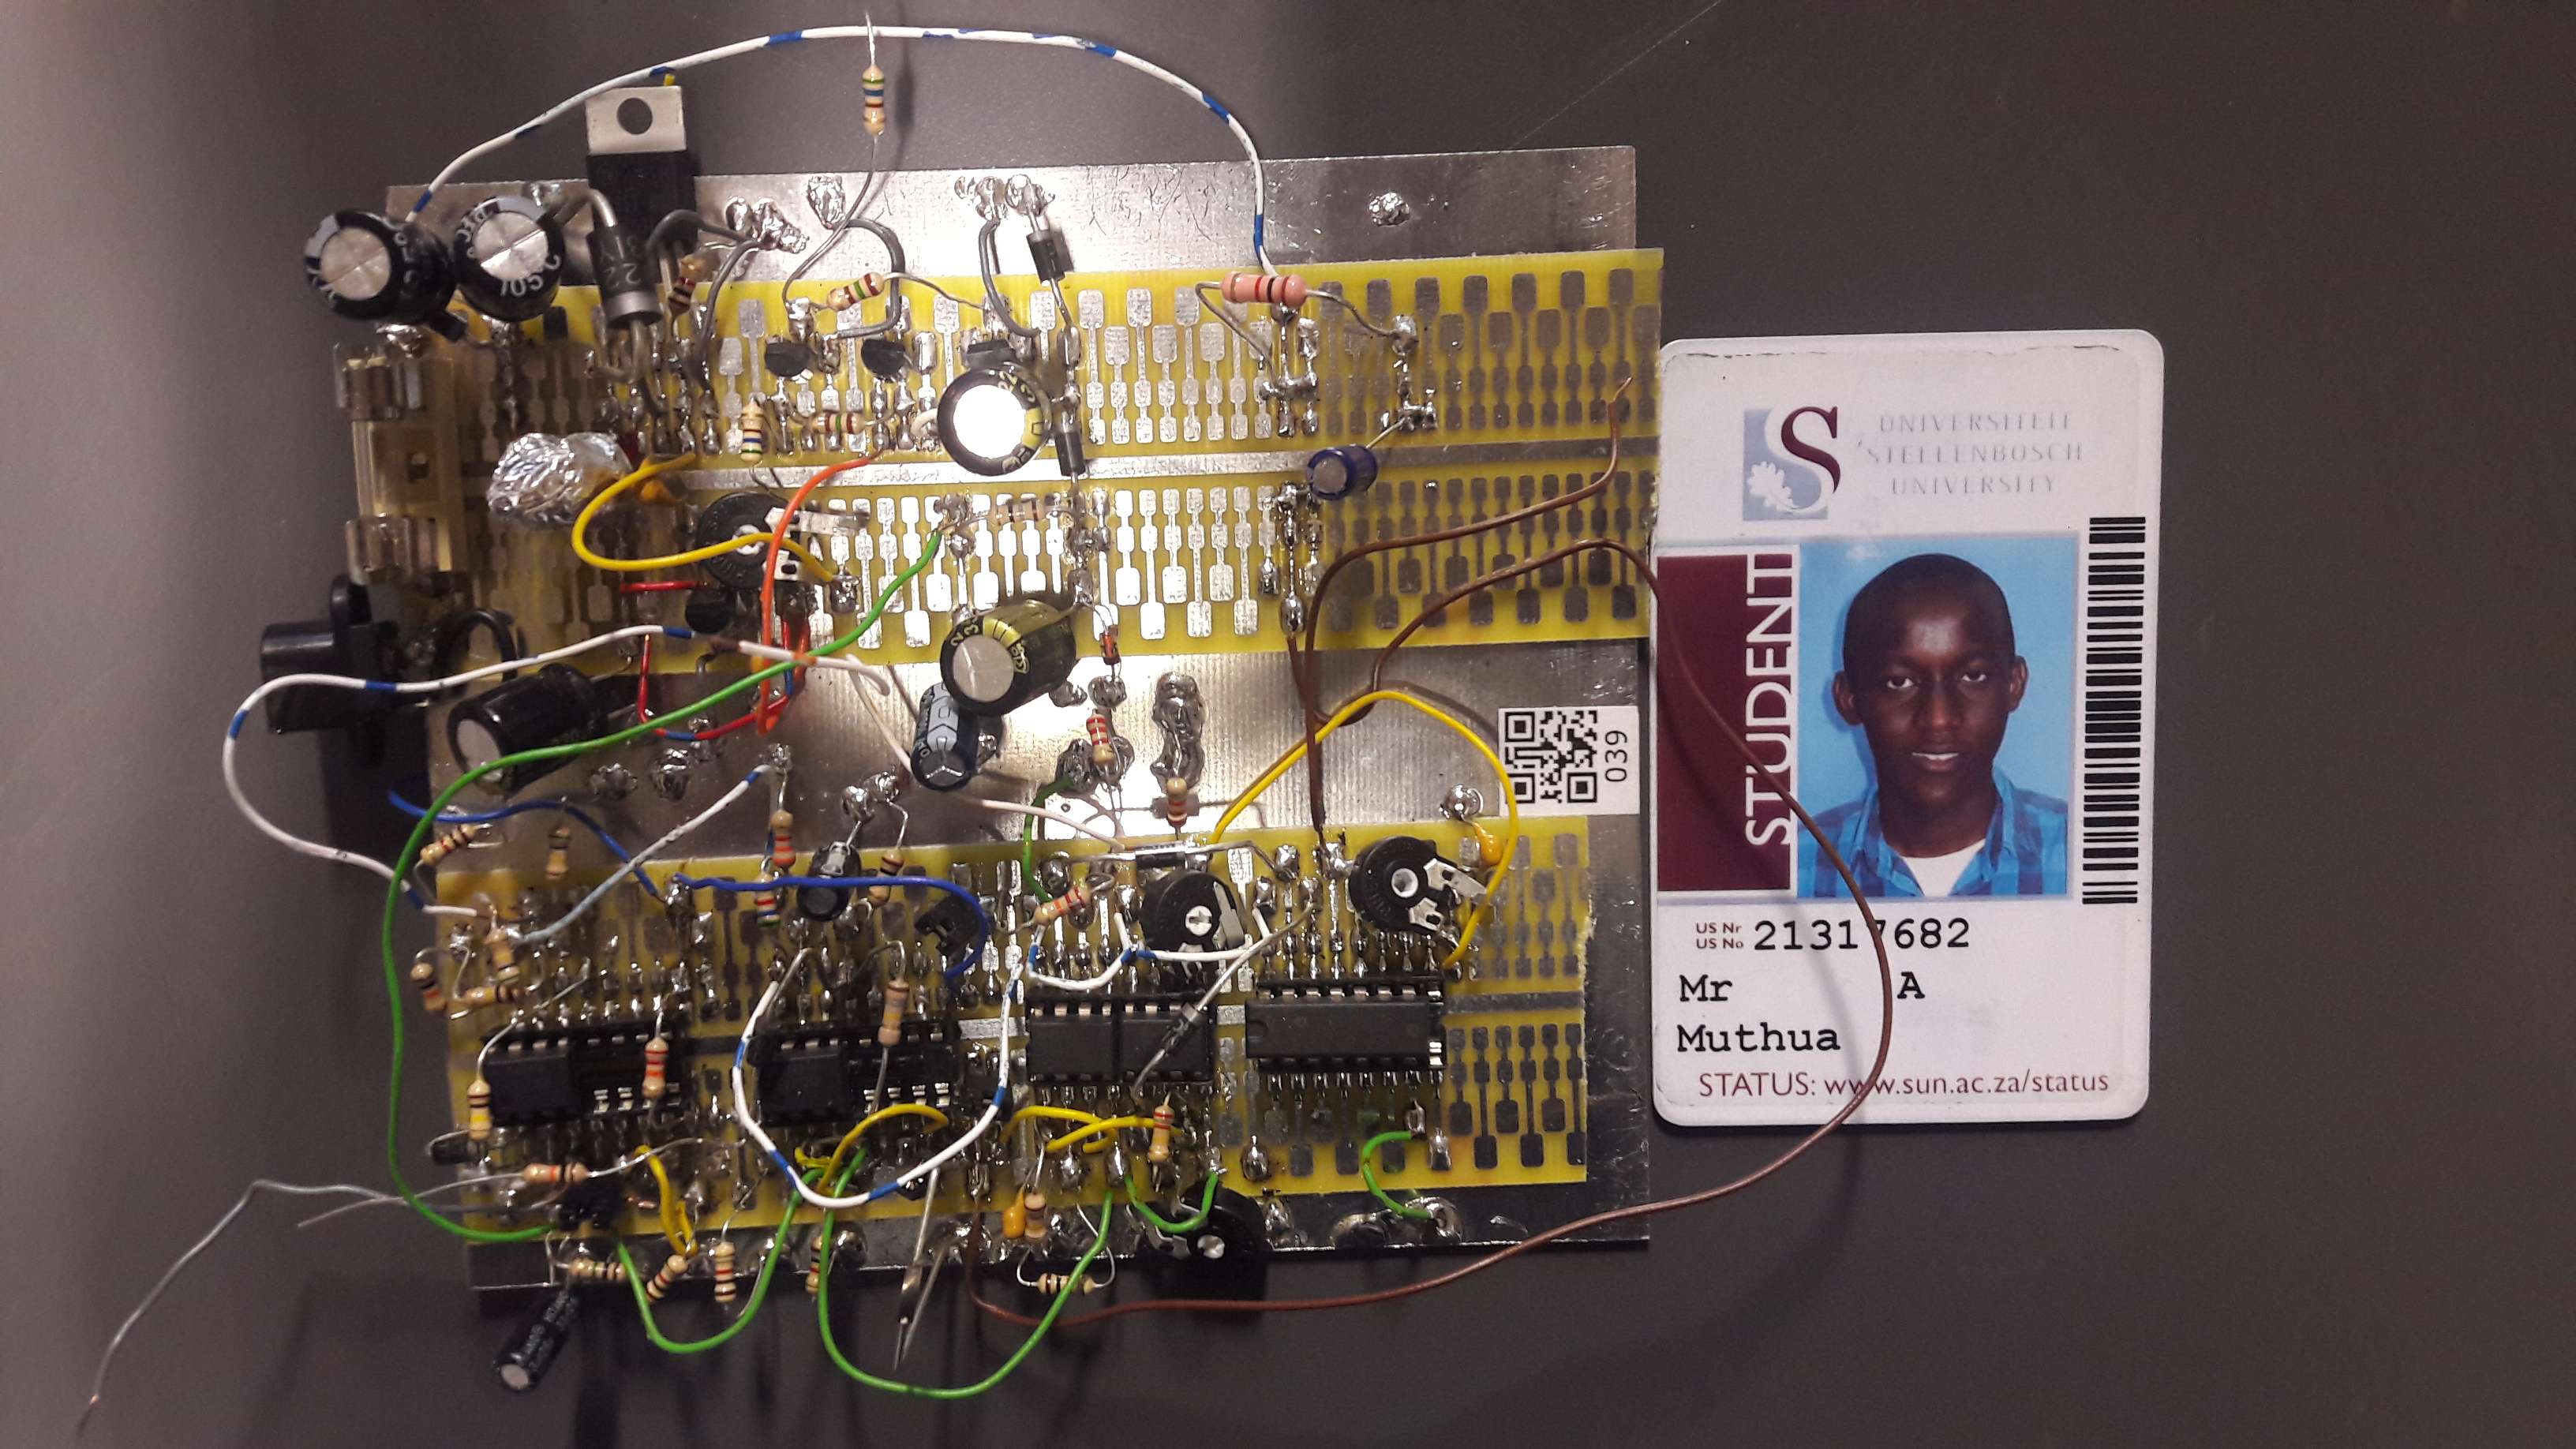
\includegraphics[width=0.5\linewidth]{./Figures/Assignment2_PCB}
		    \caption{Assignment 2 PCB.} \label{fig:pcb}
 \end{figure}
 
 \begin{figure}
 \centering
     \begin{subfigure}[]{0.35\textwidth}
        \centering
         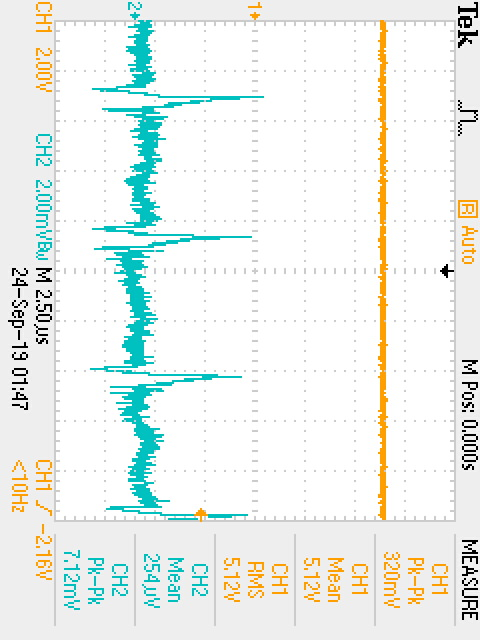
\includegraphics[height=1\linewidth, angle=90]{./Figures/+5V}
		    \caption{+5V rail with noise level.} \label{subfig:+5v_rail}
     \end{subfigure}
      \begin{subfigure}[]{0.35\textwidth}
              \centering
  		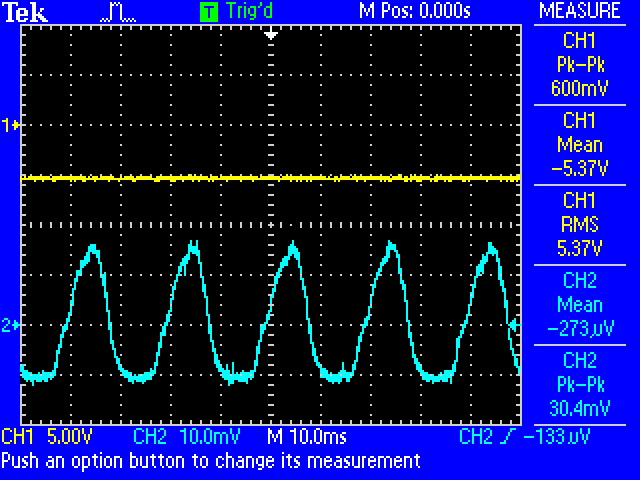
\includegraphics[width=1\linewidth]{./Figures/-5V}
		    \caption{-5V rail with noise level.} \label{subfig:-5v_rail}
     \end{subfigure}
   \caption{Noise and rail voltages with all three systems running together.}
    \label{fig:rails}
 \end{figure}
 
 
By using a multimeter in series with both the +5V and -5V supply, it is measured that the system draws $\SI{8.38}{\milli\ampere}$ from the +5V supply and $\SI{6.84}{\milli\ampere}$ from the negative rail. This is lower than the estimation in Section \ref{sec:system}.








